\documentclass[tikz]{standalone}
\usepackage{amsmath}
\usepackage{pgfplots}
\usepackage{times}
\usepackage{txfonts}
\usetikzlibrary{arrows,intersections,math}

\begin{document}
	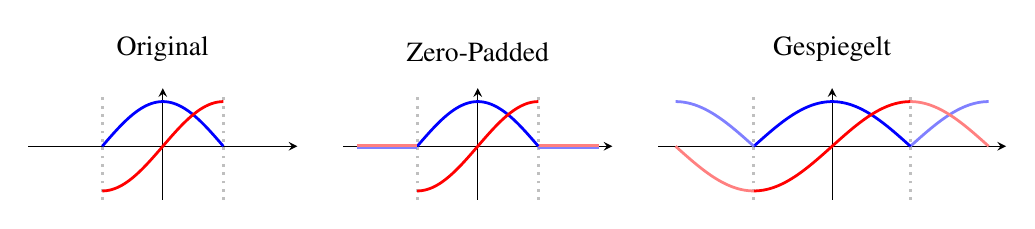
\begin{tikzpicture}
	\begin{scope}
	\begin{axis}[axis lines=middle, width=5cm, height=3cm, title={Original},
	y label style={at={(axis cs:0.2, 1)},anchor=west},
	xmin=-200, xmax=200, ymin=-1.2, ymax=1.3, ytick={-2}, xtick={-2000}]
	
		\draw[line width=1pt, dotted, gray, opacity=0.5] (axis cs:-90,-1.2) -- (axis cs:-90,1.2);
		\draw[line width=1pt, dotted, gray, opacity=0.5] (axis cs: 90,-1.2) -- (axis cs: 90,1.2);
	
		\addplot[domain= -90:90, samples=50, smooth, line width=1pt, color=blue] {cos(\x)};
		\addplot[domain= -90:90, samples=50, smooth, line width=1pt, color=red ] {sin(\x)};
		
	\end{axis}
	\end{scope}
	\begin{scope}[xshift=4cm]
	\begin{axis}[axis lines=middle, width=5cm, height=3cm, title={Zero-Padded},
	xmin=-200, xmax=200, ymin=-1.2, ymax=1.3, ytick={-2}, xtick={-2000}]
	
		\draw[line width=1pt, dotted, gray, opacity=0.5] (axis cs:-90,-1.2) -- (axis cs:-90,1.2);
		\draw[line width=1pt, dotted, gray, opacity=0.5] (axis cs: 90,-1.2) -- (axis cs: 90,1.2);

		\addplot[domain= 90:180, samples=50, smooth, line width=1pt, color=blue!50] {-0.025};
		\addplot[domain= 90:180, samples=50, smooth, line width=1pt, color=red!50 ] { 0.025};

		\addplot[domain= -90:90, samples=50, smooth, line width=1pt, color=blue] {cos(\x)};
		\addplot[domain= -90:90, samples=50, smooth, line width=1pt, color=red ] {sin(\x)};
		
		\addplot[domain= -180:-90, samples=50, smooth, line width=1pt, color=blue!50] {-0.025};
		\addplot[domain= -180:-90, samples=50, smooth, line width=1pt, color=red!50 ] { 0.025};
	
	\end{axis}
	\end{scope}
	\begin{scope}[xshift=8cm]
	\begin{axis}[axis lines=middle, width=6cm, height=3cm, title={Gespiegelt},
	xmin=-200, xmax=200, ymin=-1.2, ymax=1.3, ytick={-2}, xtick={-2000}]
	
		\draw[line width=1pt, dotted, gray, opacity=0.5] (axis cs:-90,-1.2) -- (axis cs:-90,1.2);
		\draw[line width=1pt, dotted, gray, opacity=0.5] (axis cs: 90,-1.2) -- (axis cs: 90,1.2);

		\addplot[domain= 90:180, samples=50, smooth, line width=1pt, color=blue!50] {cos(180-\x)};
		\addplot[domain= 90:180, samples=50, smooth, line width=1pt, color=red!50 ] {sin(180-\x)};

		\addplot[domain= -90:90, samples=50, smooth, line width=1pt, color=blue] {cos(\x)};
		\addplot[domain= -90:90, samples=50, smooth, line width=1pt, color=red ] {sin(\x)};
		
		\addplot[domain= -180:-90, samples=50, smooth, line width=1pt, color=blue!50] {cos(-180-\x)};
		\addplot[domain= -180:-90, samples=50, smooth, line width=1pt, color=red!50 ] {sin(-180-\x)};
	
	\end{axis}
	\end{scope}
%	\begin{scope}[yshift=-2.5 cm, xshift=6cm]
%	\begin{axis}[axis lines=middle, width=7cm, height=3cm, title={Gespiegelt, Konjugiert-Komplex},
%	xmin=-200, xmax=200, ymin=-1.2, ymax=1.3, ytick={-2}, xtick={-2000}]
%	
%		\draw[line width=1pt, dotted, gray, opacity=0.5] (axis cs:-90,-1.2) -- (axis cs:-90,1.2);
%		\draw[line width=1pt, dotted, gray, opacity=0.5] (axis cs: 90,-1.2) -- (axis cs: 90,1.2);
%
%		\addplot[domain= 90:180, samples=50, smooth, line width=1pt, color=blue!50] {cos(180-\x)};
%		\addplot[domain= 90:180, samples=50, smooth, line width=1pt, color=red!50 ] {-sin(180-\x)};
%
%		\addplot[domain= -90:90, samples=50, smooth, line width=1pt, color=blue] {cos(\x)};
%		\addplot[domain= -90:90, samples=50, smooth, line width=1pt, color=red ] {sin(\x)};
%		
%		\addplot[domain= -180:-90, samples=50, smooth, line width=1pt, color=blue!50] {cos(-180-\x)};
%		\addplot[domain= -180:-90, samples=50, smooth, line width=1pt, color=red!50 ] {-sin(-180-\x)};
%	
%	\end{axis}
%	\end{scope}
	\end{tikzpicture}
\end{document}
